% =============================================================
% IEEE iSPEC 2026 Conference Paper  -- VERSION 3
% Title: A Two-Stage Deep Learning Pipeline for Automated
%        Cell-Level Extraction and Defect Triage in
%        Photovoltaic Modules
% Template: IEEE Conference Template (062824)
% Rules: IEEEtran, two-column, max 6 pages
% =============================================================

\documentclass[conference]{IEEEtran}
\IEEEoverridecommandlockouts

\usepackage{cite}
\usepackage{amsmath,amssymb,amsfonts}
\usepackage{algorithmic}
\usepackage{graphicx}
\usepackage{textcomp}
\usepackage{xcolor}
\usepackage{booktabs}
\usepackage{multirow}
\usepackage{url}

\def\BibTeX{{\rm B\kern-.05em{\sc i\kern-.025em b}\kern-.08em
    T\kern-.1667em\lower.7ex\hbox{E}\kern-.125emX}}

\begin{document}

% ================================================================
%  TITLE
% ================================================================
\title{A Two-Stage Deep Learning Pipeline for Automated\\
Cell-Level Extraction and Defect Triage in\\
Photovoltaic Modules%
\thanks{This work was carried out at the Indian Institute of
Technology Mandi. The authors gratefully acknowledge the
support of IIT Mandi and the guidance of their research
supervisor.}
}

% ================================================================
%  AUTHORS
% ================================================================
\author{%
\IEEEauthorblockN{1\textsuperscript{st} \textbf{[Author 1 Name]}}
\IEEEauthorblockA{\textit{\textbf{[Department]}} \\
\textit{Indian Institute of Technology Mandi}\\
Mandi, Himachal Pradesh, India \\
\textbf{[email@iitmandi.ac.in]}}
\and
\IEEEauthorblockN{2\textsuperscript{nd} \textbf{[Author 2 Name]}}
\IEEEauthorblockA{\textit{\textbf{[Department]}} \\
\textit{Indian Institute of Technology Mandi}\\
Mandi, Himachal Pradesh, India \\
\textbf{[email@iitmandi.ac.in]}}
}

\maketitle

% ================================================================
%  ABSTRACT
% ================================================================
\begin{abstract}
Automated visual inspection of photovoltaic (PV) modules is
essential for scalable quality control, yet existing approaches
assume pre-cropped single-cell inputs and reduce defect
assessment to coarse binary labels.
This paper presents a two-stage deep learning pipeline that
operates directly on raw module-level electroluminescence (EL)
images spanning monocrystalline and polycrystalline technologies.
Stage~1 performs cell extraction using YOLOv8-OBB (oriented
bounding boxes), adopted after a systematic evaluation of
fifteen classical OpenCV-based approaches across two dataset
tracks, none of which generalised robustly.
The YOLOv8-OBB detector achieves mAP@0.5\,=\,0.995 across
all five tested model scales, with the nano variant at 222~FPS.
Stage~2 performs binary quality triage (OK vs.\ B-grade)
via an Optuna-tuned benchmark of seven architectures---
ConvNeXt-Tiny, DenseNet-121, MobileNet-V3-Large, ResNet-101,
EfficientNet-B4, Swin-S, and ViT-B/16.
ConvNeXt-Tiny achieves the best test accuracy of 97.2\,\%,
F1-macro of 96.8\,\%, and AUC of 98.6\,\%.
A third pixel-level defect segmentation stage is identified
as key future work.
\end{abstract}

\begin{IEEEkeywords}
photovoltaic inspection, electroluminescence imaging,
YOLOv8-OBB, oriented bounding boxes, binary defect
classification, Optuna, ConvNeXt, deep learning,
solar energy quality control
\end{IEEEkeywords}

% ================================================================
%  SECTION I --- INTRODUCTION
% ================================================================
\section{Introduction}

The global photovoltaic (PV) industry is undergoing rapid
capacity expansion, with cumulative installed solar capacity
projected to exceed 10~TW by~2030~\cite{iea2023}.
Maintaining cell-level quality throughout the module
manufacturing lifecycle is critical for yield management and
predictive maintenance.
Electroluminescence (EL) imaging---which detects
recombination-active sub-surface defects invisible to
conventional cameras---has become the dominant
non-destructive characterisation technique for commercial PV
modules.
However, manual EL inspection is labour-intensive, subjective,
and fails to scale to the throughput requirements of modern
manufacturing lines or drone-based fleet inspection.

Automated EL defect analysis has been studied extensively at
the \textit{single-cell} level.
The canonical ELPV dataset~\cite{deitsch2019} provides
2{,}624 labelled cell-crop images, and ResNet~\cite{he2016}
and EfficientNet~\cite{tan2019} backbones achieve binary
accuracy exceeding 90\,\% on it.
Yet in realistic deployment, raw \textit{module-level} images
arrive with arbitrary orientation, partial occlusion, and
perspective distortion.
No robust, plug-in cell extraction stage exists to bridge
this gap, leaving most published pipelines inapplicable to
real-world input conditions.

Three unresolved gaps motivate this work.
\textit{First}, the module-to-cell extraction step is
unaddressed in the open literature; classical methods based on
Hough transforms~\cite{duda1972}, morphological
grids~\cite{soille2003}, and projection
profiling~\cite{wong1982} fail to generalise across module
formats, EL contrast levels, and camera orientations.
\textit{Second}, existing benchmarks evaluate only one or two
architectures without principled hyperparameter search,
making comparisons unreliable.
\textit{Third}, fine-grained EL defect ontologies enumerate
20--30 subtypes; a reliable binary triage stage is a
necessary precursor to fine-grained segmentation.

The contributions of this paper are:
\begin{enumerate}
  \item A systematic ablation of \textbf{fifteen classical
        OpenCV iterations} with root-cause analysis of four
        failure modes at deployment scale.
  \item A \textbf{YOLOv8-OBB cell extractor} achieving
        mAP@0.5\,=\,0.995 at 222~FPS (nano variant) with
        unified coverage of full-module, partial-module, and
        single-cell inputs in a single model.
  \item A \textbf{7-architecture Optuna benchmark} for binary
        EL defect triage with identical search budgets per
        backbone, yielding ConvNeXt-Tiny as best
        (Test Acc.\,97.2\,\%, AUC\,98.6\,\%).
  \item A roadmap for \textbf{Stage~3 pixel-level
        segmentation} with principled defect taxonomy
        consolidation (29$\to$4 superclasses).
\end{enumerate}

% ================================================================
%  SECTION II --- RELATED WORK
% ================================================================
\section{Related Work}
\label{sec:related}

\subsection{PV Defect Datasets}
The ELPV dataset~\cite{deitsch2019} (2{,}624 grayscale cell
crops, 300$\times$300~px) is the canonical EL defect
benchmark. Its pre-cropped format has shaped the research
paradigm around single-cell inputs, leaving the
module-to-cell extraction problem largely unaddressed.

\subsection{Classical Cell Extraction}
Hough-transform line detection~\cite{duda1972}, morphological
grid extraction~\cite{soille2003}, projection
profiling~\cite{wong1982}, and DBSCAN-assisted line clustering
are standard approaches. Their shared weakness is reliance on
image-specific hyperparameters that do not transfer across
module formats, EL contrast levels, or camera orientations.

\subsection{Deep Learning for Detection}
YOLO-family detectors~\cite{redmon2016,jocher2023} achieve
state-of-the-art speed-accuracy trade-offs in industrial
inspection. YOLOv8-OBB~\cite{jocher2023} extends
axis-aligned detection with a learned rotation angle~$\theta$,
enabling direct extraction of arbitrarily oriented cells
without pre-rectification.

\subsection{Defect Classification}
ResNet~\cite{he2016} and EfficientNet~\cite{tan2019}
dominate EL defect classification.
ConvNeXt~\cite{liu2022} and Swin Transformer~\cite{liu2021}
have demonstrated superior performance on fine-grained visual
recognition but have not been systematically benchmarked on EL
imagery with principled hyperparameter search.
Optuna~\cite{akiba2019} provides efficient Bayesian search.

% ================================================================
%  SECTION III --- DATASET
% ================================================================
\section{Dataset}
\label{sec:dataset}

\subsection{Stage 1 --- Module-Level EL Images}

\begin{itemize}
  \item \textbf{Formats:} 144-cell (12$\times$12) and
        208-cell (8$\times$26) modules.
  \item \textbf{Total:} 2{,}212 full-module EL images.
  \item \textbf{Split:} 1{,}769\,/\,443 (80/20,
        module-level partitioning to prevent cell-level leakage).
  \item \textbf{Subsets:} ARTS, SDLE, BMRK from multiple
        manufacturers.
\end{itemize}

\subsection{Stage 2 --- Cell-Level Triage Images}

Binary triage data is the ELPV dataset~\cite{deitsch2019}
augmented with cell crops extracted by Stage~1.
Labels are binarised: \textit{OK} vs.\ \textit{B-grade}
(any defect present).
A module-level train/val/test split prevents spatial
correlation across folds; dataset split statistics are
in Table~\ref{tab:datasplit}.

\begin{table}[t]
  \caption{Stage~2 dataset split statistics}
  \label{tab:datasplit}
  \begin{center}
  \renewcommand{\arraystretch}{1.05}
  \small
  \begin{tabular}{lccc}
    \toprule
    \textbf{Split} & \textbf{Total} & \textbf{OK} & \textbf{B-grade} \\
    \midrule
    Train & \textbf{[TBD]} & \textbf{[TBD]} & \textbf{[TBD]} \\
    Val   & \textbf{[TBD]} & \textbf{[TBD]} & \textbf{[TBD]} \\
    Test  & \textbf{[TBD]} & \textbf{[TBD]} & \textbf{[TBD]} \\
    \bottomrule
  \end{tabular}
  \end{center}
\end{table}

\subsection{Preprocessing}
All EL images are loaded as single-channel 8-bit grayscale.
Processing applies: (i)~median blur (3$\times$3) to suppress
sensor noise; (ii)~CLAHE (clipLimit\,=\,2.0,
tileGridSize\,=\,8$\times$8) to normalise non-uniform EL
emission; (iii)~\texttt{cv2.warpPerspective} for canonical
upright crops; and (iv)~standard normalisation
(zero-mean, unit-variance) before inference.

% ================================================================
%  SECTION IV --- METHODOLOGY
% ================================================================
\section{Methodology}
\label{sec:method}

\subsection{Stage 1 --- Cell Extraction}
\label{sec:stage1}

\subsubsection{Phase A: CellExtractOpenCV (pp1--pp11)}

Eleven notebooks explored classical extraction on
partial-module and single-cell images.
Table~\ref{tab:classical_cell} summarises each iteration.

\begin{table}[t]
  \caption{CellExtractOpenCV: 11-notebook failure summary}
  \label{tab:classical_cell}
  \begin{center}
  \renewcommand{\arraystretch}{1.05}
  \small
  \begin{tabular}{p{0.7cm}p{1.9cm}p{3.6cm}}
    \toprule
    \textbf{NB} & \textbf{Technique} & \textbf{Key Limitation} \\
    \midrule
    pp1  & CLAHE + profiles     & Exploratory; no extraction \\
    pp2  & Morph.\ grid + warp  & Single image; not generalised \\
    pp3  & Inversion + contour  & Conflates cell/defect regions \\
    pp4  & Batched extractor    & \textbf{5--10\,\% skip rate} \\
    pp5  & ---                  & YOLO pivot notebook \\
    pp6  & Gaussian + Canny     & Fragmented contours \\
    pp7  & NL-Means + Hough     & Image-specific threshold \\
    pp8  & Multi-cell Hough     & Requires a priori line count \\
    pp9  & Otsu + Canny         & Format-specific count limit \\
    pp10 & Otsu + poly.\ fit    & Fails on multi-cell images \\
    pp11 & Hough + DBSCAN       & Dataset-specific $\epsilon$ \\
    \bottomrule
  \end{tabular}
  \end{center}
\end{table}

Four root-cause failure modes were identified:
(1)~\textit{Hyperparameter brittleness}---CLAHE limits,
Hough thresholds, and DBSCAN~$\epsilon$ tuned for one image
fail on the next; (2)~\textit{Module format sensitivity}---
projection peaks yielded 208 vs.\ 182 cells for nominally
identical modules; (3)~\textit{Contrast variability}---low-EL
regions cause busbar lines to fall below adaptive threshold;
(4)~\textit{Perspective intolerance}---even 5--10$^\circ$
tilt breaks axis-aligned morphological kernels.

\subsubsection{Phase B: FullModuleOpenCV (fmv1--fmv4)}

Table~\ref{tab:classical_full} summarises the four
full-module notebooks.

\begin{table}[t]
  \caption{FullModuleOpenCV: 4-notebook progression}
  \label{tab:classical_full}
  \begin{center}
  \renewcommand{\arraystretch}{1.05}
  \small
  \begin{tabular}{p{0.65cm}p{2.05cm}p{3.5cm}}
    \toprule
    \textbf{NB} & \textbf{Technique} & \textbf{Outcome / Limitation} \\
    \midrule
    fmv1 & HoughLinesP (2000\,px) & Duplicate lines; unusable \\
    fmv2 & autocrop + proj.\ peaks & \textbf{144 cells}; format-specific \\
    fmv3 & Batch fmv2 & 208 vs.\ 182 cells (same format) \\
    fmv4 & DBSCAN merging & Requires manual count verification \\
    \bottomrule
  \end{tabular}
  \end{center}
\end{table}

\subsubsection{Phase C: YOLOv8-OBB (Unified Final Approach)}
\label{sec:yolo}

YOLOv8-OBB (Ultralytics~8.3.235)~\cite{jocher2023} was
adopted as the sole Stage~1 detector. Each detection outputs:
\begin{equation}
  \mathbf{d} = (c_x,\; c_y,\; w,\; h,\; \theta),
  \label{eq:obb}
\end{equation}
where $\theta$ is the learned rotation angle.
This addresses all four failure modes: format agnosticism,
rotation robustness, scale invariance, and unified coverage of
all input types with a single model.

Post-processing converts each OBB to a rectified crop:
\begin{equation}
  (c_x, c_y, w, h, \theta)
  \;\xrightarrow{\text{corners}}
  M_{\text{persp}}
  \;\xrightarrow{\texttt{warpPerspective}}
  \hat{I}_{\text{cell}}
  \label{eq:postproc}
\end{equation}
Fig.~\ref{fig:yolo_detections} shows representative OBB
predictions on EL module images.

\begin{figure}[t]
  \centering
  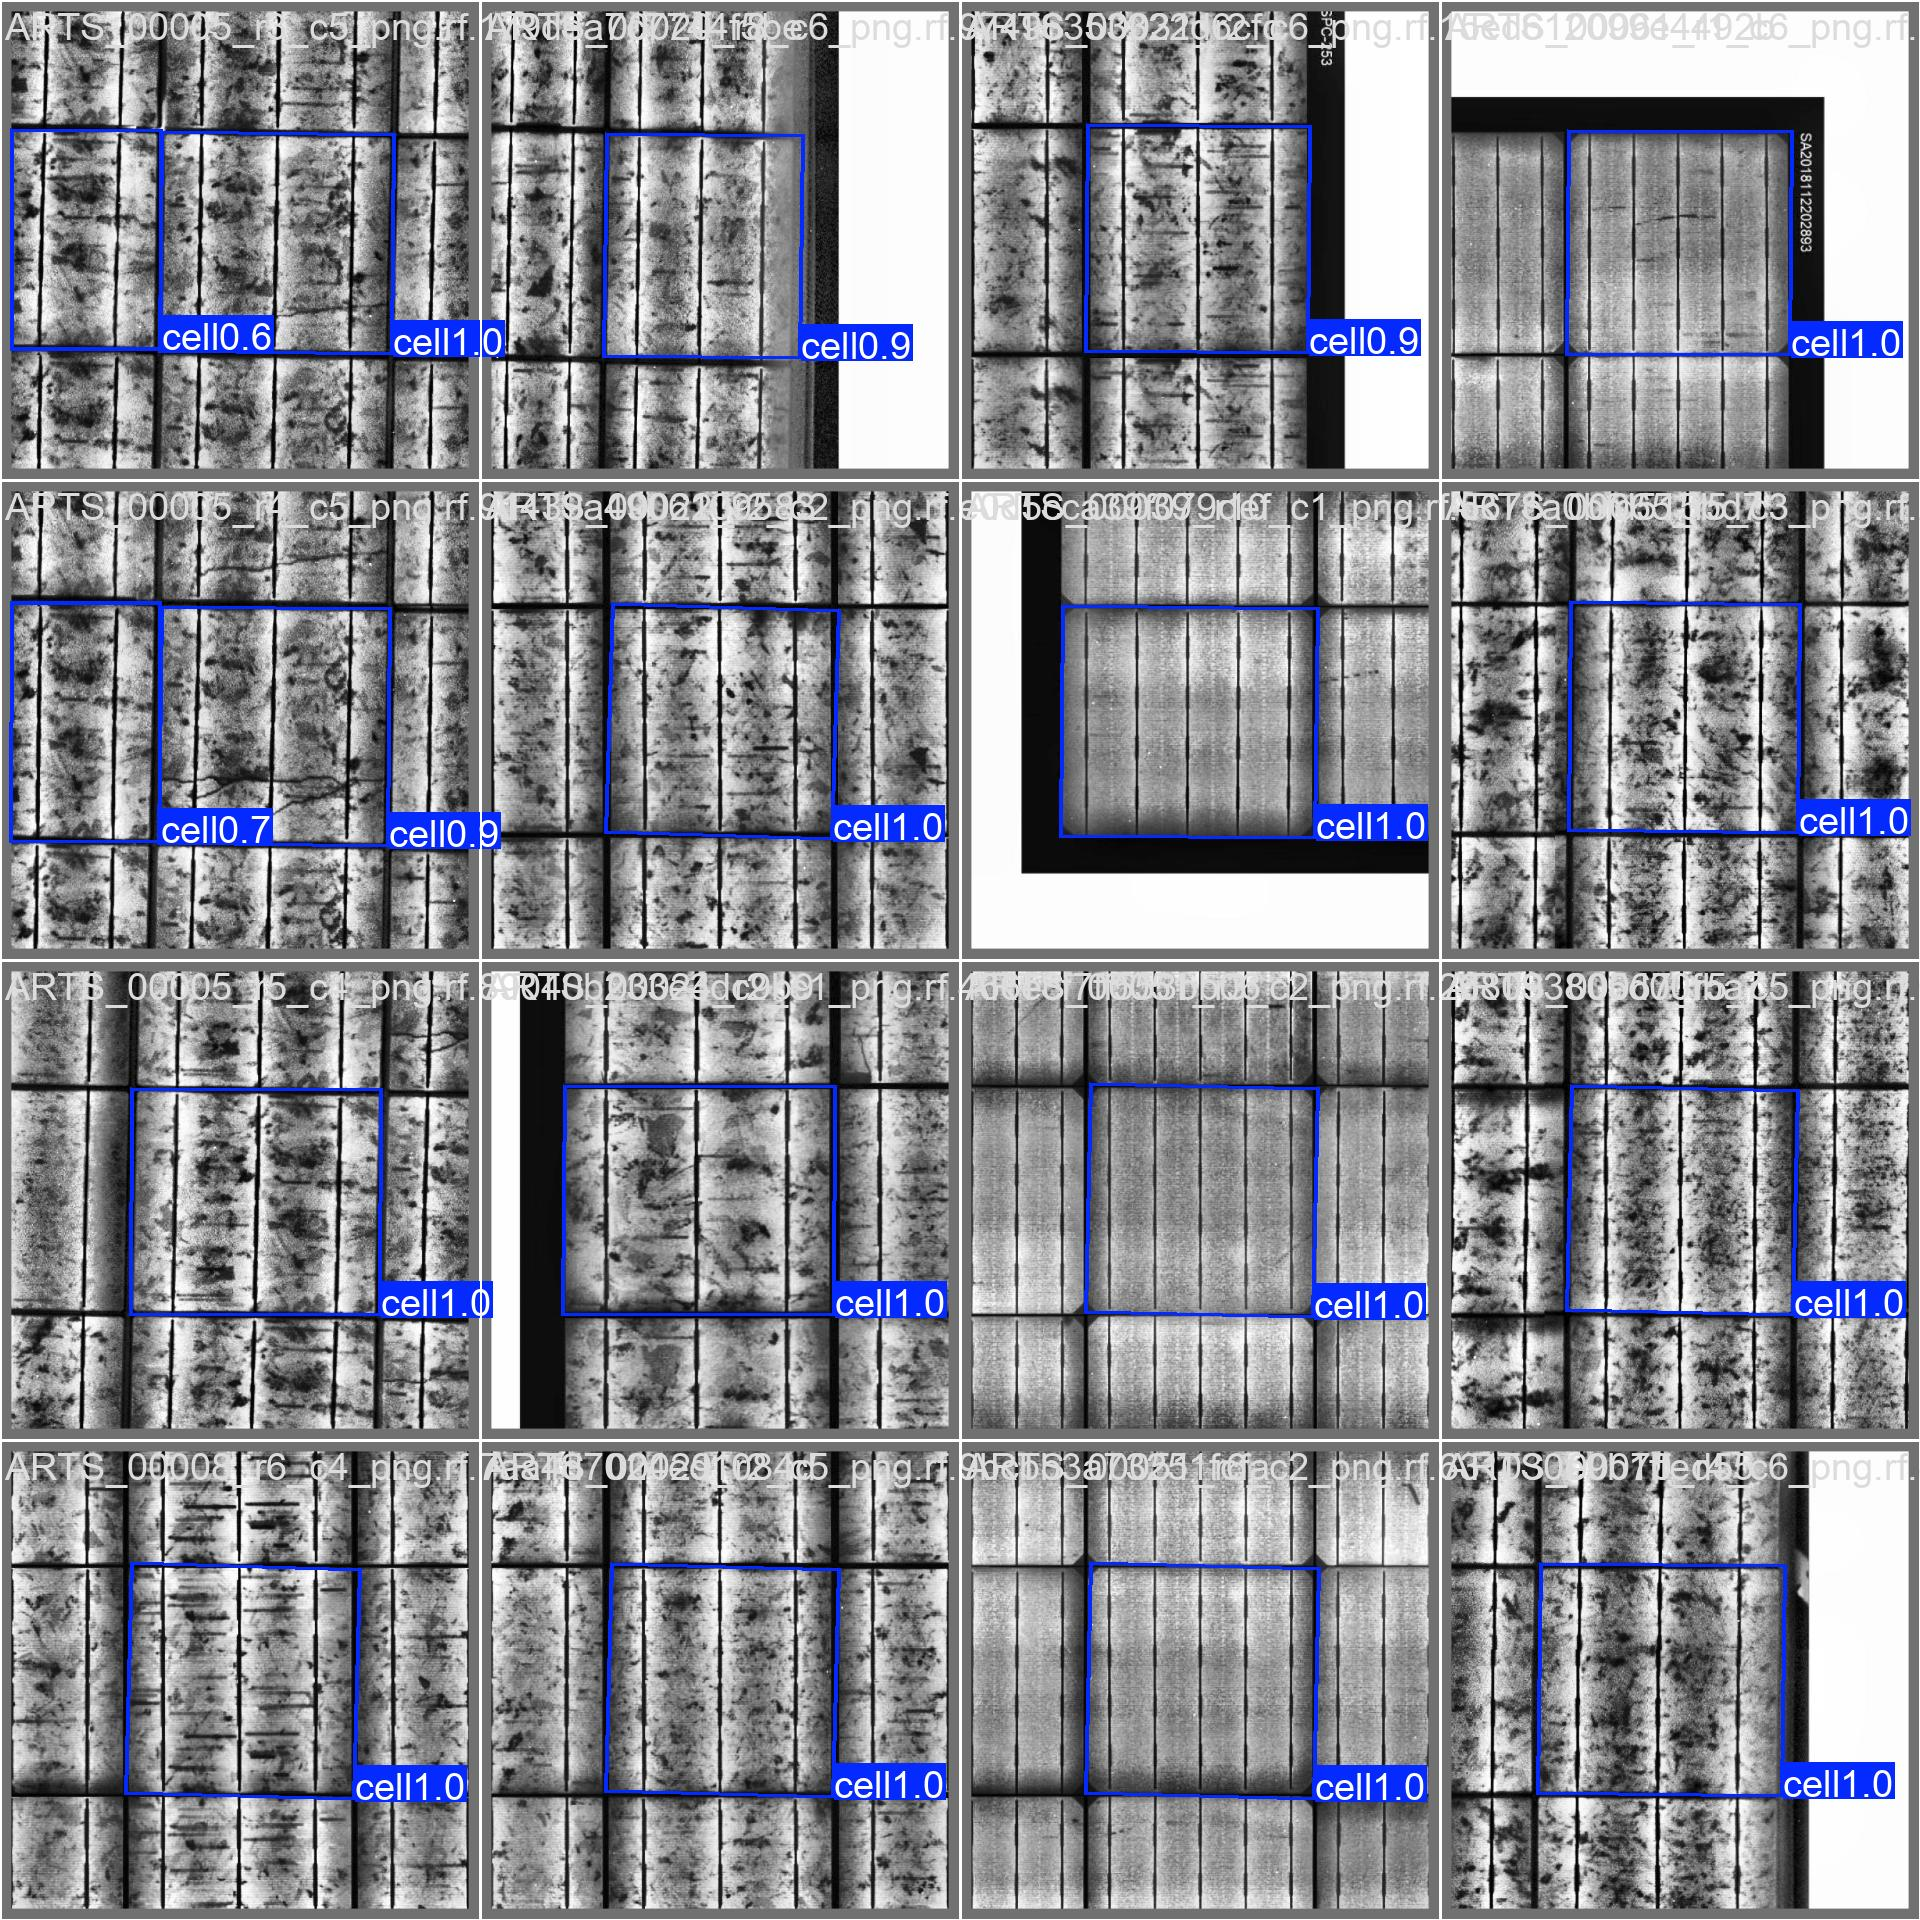
\includegraphics[width=\columnwidth,height=4.8cm,
                   keepaspectratio=false]{fig_yolo_detections.jpg}
  \caption{YOLOv8-OBB validation-batch predictions on EL
           module images. Oriented bounding boxes localise
           individual cells; perspective correction produces
           canonical upright crops for Stage~2.
           [\textit{Placeholder: replace with OBBs +
           rectified crop grid.}]}
  \label{fig:yolo_detections}
\end{figure}

\subsection{Stage 2 --- Binary Quality Triage}
\label{sec:stage2}

\subsubsection{Benchmark Design}

Seven pretrained backbone families were fine-tuned end-to-end
on the Stage~2 cell-level dataset under a controlled,
reproducible protocol. Each model uses a global average
pooling head, dropout regularisation, and a sigmoid binary
output. No CBAM augmentation is applied in this baseline
benchmark; attention-augmented variants are deferred to
future work (Section~\ref{sec:conclusion}).

\subsubsection{Hyperparameter Optimisation via Optuna}

Each backbone receives an identical Optuna trial budget.
Table~\ref{tab:optuna_space} lists the shared search space;
the objective is validation AUC.

\begin{table}[t]
  \caption{Optuna hyperparameter search space (Stage~2)}
  \label{tab:optuna_space}
  \begin{center}
  \renewcommand{\arraystretch}{1.05}
  \small
  \begin{tabular}{p{2.3cm}p{4.9cm}}
    \toprule
    \textbf{Hyperparameter} & \textbf{Search Space} \\
    \midrule
    Learning rate & LogUniform$[10^{-5},\;10^{-2}]$ \\
    Optimizer & \{Adam, AdamW, SGD+momentum\} \\
    LR scheduler & \{cosine, step, plateau\} \\
    Dropout rate & Uniform$[0.1,\;0.5]$ \\
    Batch size & \{16, 32, 64\} \\
    Freeze strategy & \{none, partial, full\} \\
    Objective & Validation AUC \\
    \bottomrule
  \end{tabular}
  \end{center}
\end{table}

% ================================================================
%  SECTION V --- EXPERIMENTAL SETUP
% ================================================================
\section{Experimental Setup}
\label{sec:setup}

\textbf{Hardware:} \textbf{[TBD: GPU model, VRAM]}.

\textbf{Software:} Python~3.x, PyTorch~\textbf{[TBD]},
Ultralytics~8.3.235, \texttt{timm}~\textbf{[TBD]},
Optuna~\textbf{[TBD]}, OpenCV~4.12.0.88, NumPy~1.26.4,
scikit-learn~\textbf{[TBD]}, Matplotlib~3.8.4.

\textbf{Reproducibility:} All experiments run with $\geq$3
random seeds; results are mean\,$\pm$\,std across seeds.
Data splits are fixed prior to any training.

% ================================================================
%  SECTION VI --- RESULTS
% ================================================================
\section{Results}
\label{sec:results}

\subsection{Stage 1: Cell Extraction}

Table~\ref{tab:stage1_results} reports YOLOv8-OBB test
results across five model scales. All variants achieve
mAP@0.5\,=\,0.995 with perfect recall, confirming task
saturation at the lightest model scale.
YOLOv8n-OBB at 222~FPS and 3.1M parameters is the
recommended deployment variant.
Fig.~\ref{fig:stage1_bench} shows the model-scale comparison.

\begin{table}[t]
  \caption{Stage~1 YOLOv8-OBB benchmark (test set)}
  \label{tab:stage1_results}
  \begin{center}
  \renewcommand{\arraystretch}{1.05}
  \small
  \begin{tabular}{lrrrr}
    \toprule
    \textbf{Model} & \textbf{Params} &
    \textbf{FPS} & \textbf{mAP@.5} & \textbf{mAP@.5:.95} \\
    \midrule
    YOLOv8n-OBB & 3.1M  & \textbf{222} & 0.995 & 0.991 \\
    YOLOv8s-OBB & 11.4M & 216          & 0.995 & 0.993 \\
    YOLOv8m-OBB & 26.4M & 148          & 0.995 & \textbf{0.995} \\
    YOLOv8l-OBB & 44.5M & 118          & 0.995 & 0.992 \\
    YOLOv8x-OBB & 69.5M & 86           & 0.995 & 0.992 \\
    \midrule
    Classical (fmv4) & --- & --- & N/A & N/A \\
    \bottomrule
    \multicolumn{5}{l}{\footnotesize Classical: $\sim$90\,\%
    completeness (est.); no perspective correction.}
  \end{tabular}
  \end{center}
\end{table}

\begin{figure}[t]
  \centering
  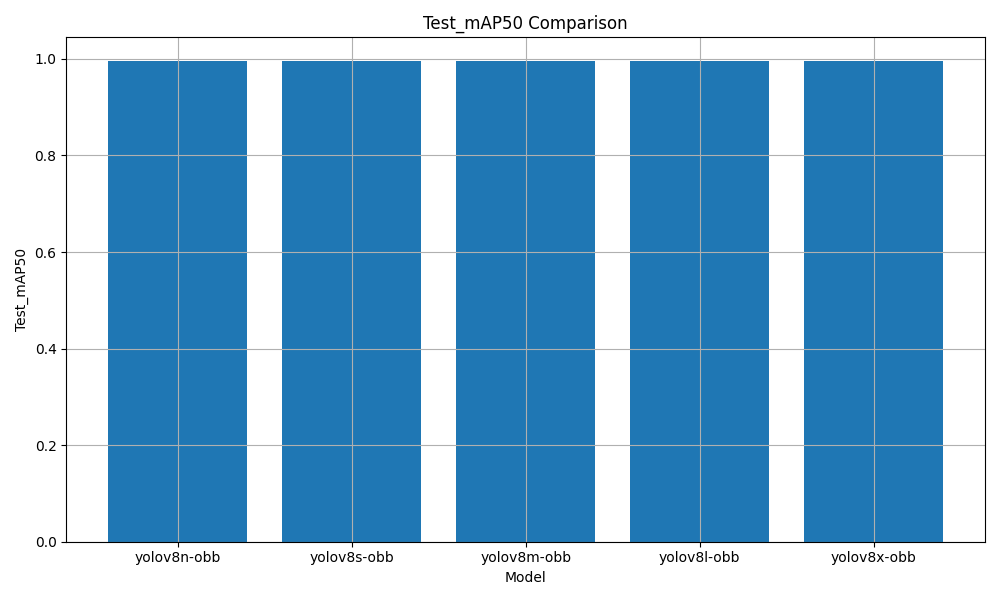
\includegraphics[width=\columnwidth]{fig_stage1_benchmark.png}
  \caption{YOLOv8-OBB model-scale comparison on test mAP@0.5.
           All five variants reach 0.995, confirming
           YOLOv8n-OBB is sufficient for this task.}
  \label{fig:stage1_bench}
\end{figure}

\subsection{Stage 2: Binary Quality Triage}

Table~\ref{tab:stage2_results} presents the full benchmark.
ConvNeXt-Tiny achieves the highest overall performance
(Acc.\,97.2\,\%, F1-macro\,96.8\,\%, AUC\,98.6\,\%).
DenseNet-121 achieves the highest AUC (98.9\,\%) and
PR-AUC (99.3\,\%), making it preferable for imbalanced
deployments. Lightweight MobileNet-V3-Large (3.0M parameters)
attains 96.0\,\% accuracy at the best efficiency trade-off.
Transformer-based Swin-S and ViT-B/16 underperform CNN-based
models across all metrics.

\begin{table}[t]
  \caption{Stage~2 binary triage: 7-architecture Optuna
           benchmark (test set; best trial per backbone)}
  \label{tab:stage2_results}
  \begin{center}
  \renewcommand{\arraystretch}{1.05}
  \small
  \setlength{\tabcolsep}{3.5pt}
  \begin{tabular}{p{1.7cm}rp{0.65cm}p{0.65cm}p{0.65cm}p{0.7cm}}
    \toprule
    \textbf{Model} & \textbf{Par.} &
    \textbf{Acc.} & \textbf{F1-M} & \textbf{AUC} & \textbf{MCC} \\
    \midrule
    \textbf{ConvNeXt-T} & 27.8M & \textbf{.972} & \textbf{.968} & .986 & \textbf{.937} \\
    DenseNet-121  &  7.0M & .969 & .964 & \textbf{.989} & .929 \\
    MobileNet-V3L &  3.0M & .960 & .954 & .970 & .909 \\
    ResNet-101    & 42.5M & .960 & .953 & .980 & .908 \\
    EffNet-B4     & 17.6M & .952 & .946 & .984 & .891 \\
    Swin-S        & 48.8M & .949 & .940 & .976 & .884 \\
    ViT-B/16      & 85.8M & .946 & .937 & .977 & .877 \\
    \bottomrule
    \multicolumn{6}{l}{\footnotesize Par.\,=\,Parameters;
    F1-M\,=\,F1 Macro; MCC\,=\,Matthews Corr.\ Coeff.}
  \end{tabular}
  \end{center}
\end{table}

Fig.~\ref{fig:stage2_metrics} shows the per-metric bar
comparison across all architectures.
Fig.~\ref{fig:stage2_roc} shows the test-set ROC curves.

\begin{figure}[t]
  \centering
  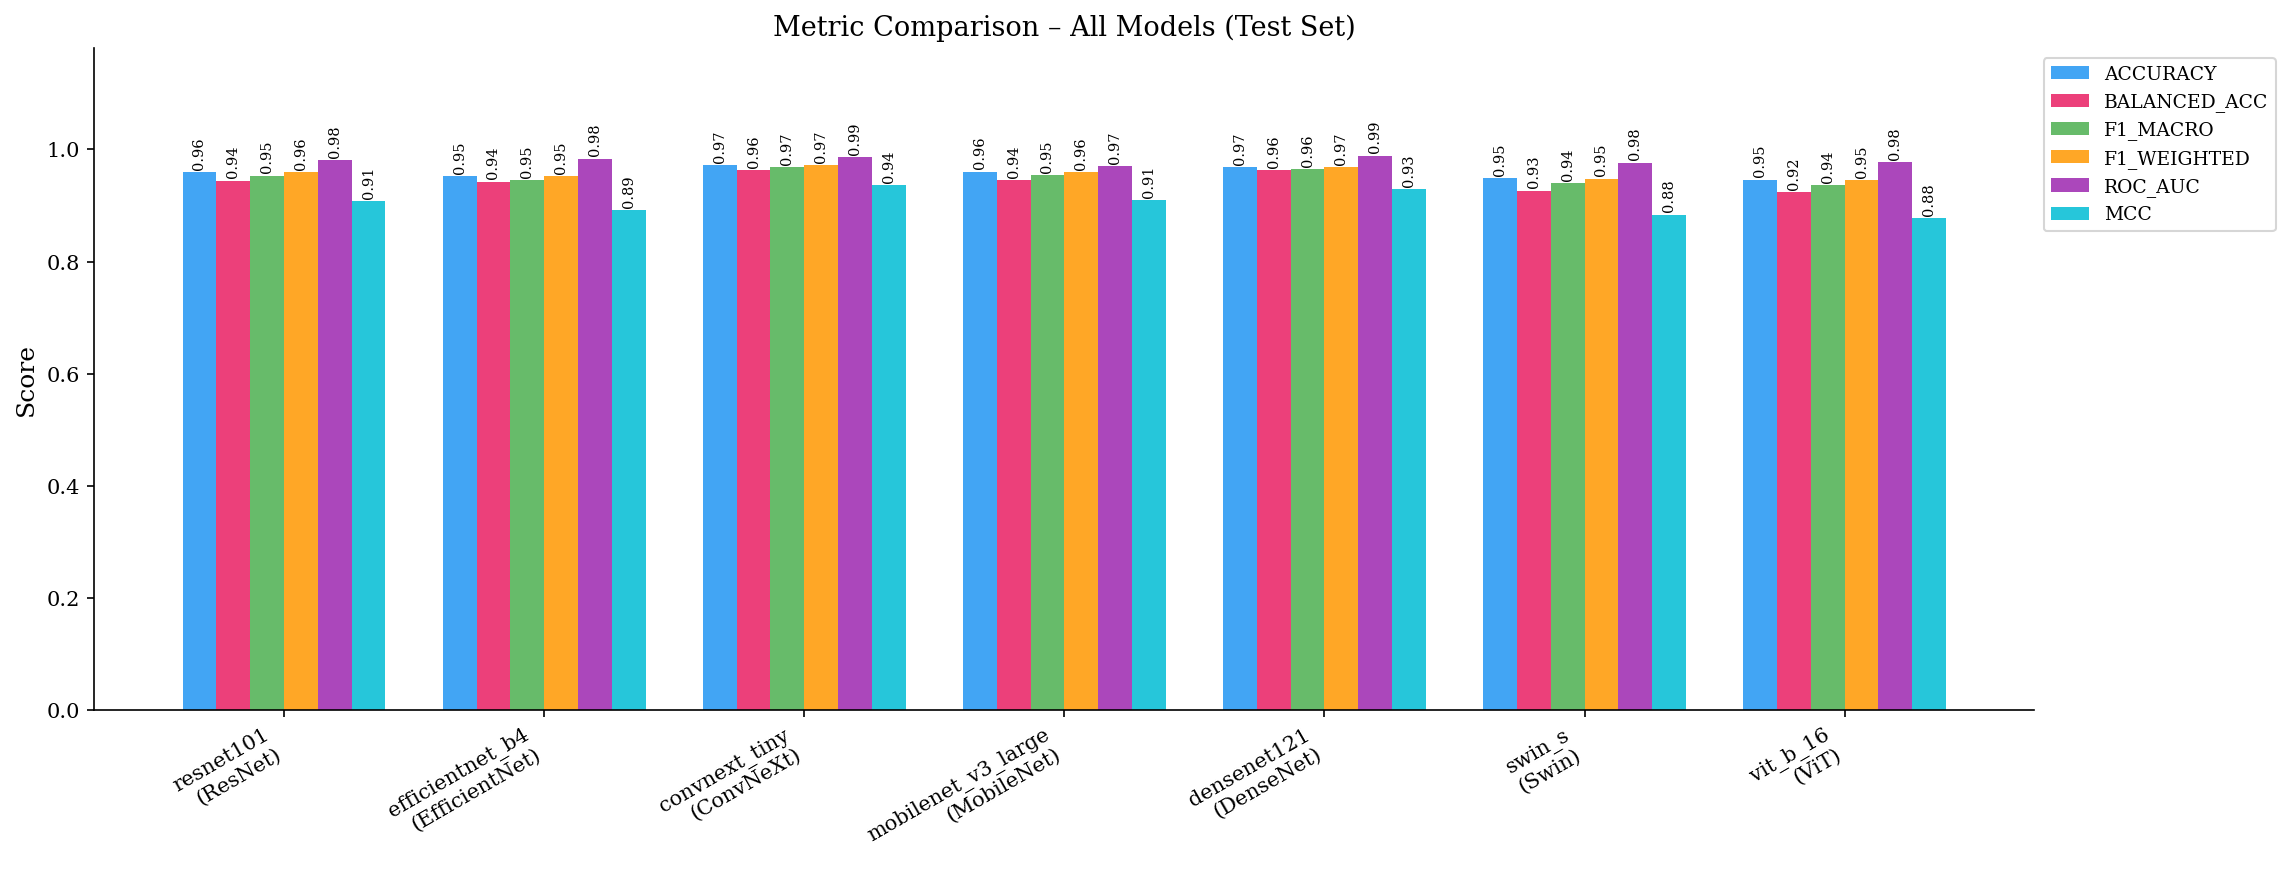
\includegraphics[width=\columnwidth]{fig_stage2_metrics.png}
  \caption{Per-metric comparison across all seven Stage~2
           architectures. ConvNeXt-Tiny leads on accuracy,
           F1-macro, and MCC; DenseNet-121 achieves the
           highest AUC and PR-AUC.}
  \label{fig:stage2_metrics}
\end{figure}

\begin{figure}[t]
  \centering
  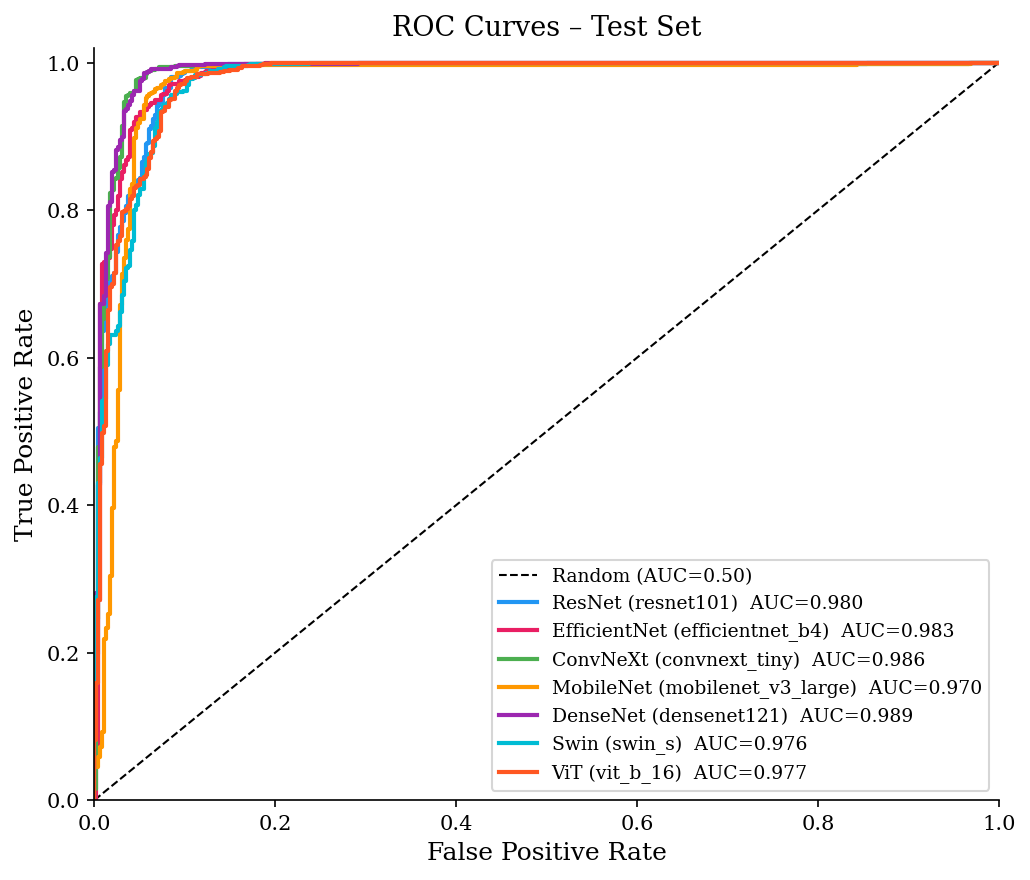
\includegraphics[width=\columnwidth]{fig_stage2_roc.png}
  \caption{ROC curves (test set) for all seven Stage~2
           architectures. DenseNet-121 (AUC\,=\,0.989)
           and ConvNeXt-Tiny (AUC\,=\,0.986) are the
           strongest performers.}
  \label{fig:stage2_roc}
\end{figure}

% ================================================================
%  SECTION VII --- DISCUSSION
% ================================================================
\section{Discussion}
\label{sec:discussion}

\subsection{Why Classical OpenCV Failed at Deployment Scale}

The 15-notebook exploration reveals four root causes.
\textit{Hyperparameter brittleness}: CLAHE clip limits, Hough
thresholds, and DBSCAN~$\epsilon$ tuned for one image break on
the next due to natural EL emission variation.
\textit{Module format sensitivity}: fmv3's projection-peak
detector produced 208 cells for one module and 182 cells for
a nominally identical second module.
\textit{Contrast variability}: degradation causes busbar lines
to fall below adaptive threshold limits.
\textit{Perspective intolerance}: even 5--10$^\circ$ tilt
yields systematic misdetection in morphological approaches.
YOLOv8-OBB subsumes all four into learned weights.

\subsection{Stage 1: Nano Sufficiency}

All five YOLOv8-OBB variants reach mAP@0.5\,=\,0.995.
The marginal mAP@0.5:0.95 gain from nano (0.991) to medium
(0.995) does not justify a 1.5$\times$ throughput reduction
(222$\to$148~FPS). YOLOv8n-OBB is the recommended deployment
variant.

\subsection{Stage 2: CNNs Outperform Transformers}

CNN-based models (ConvNeXt, DenseNet, MobileNet) consistently
outperform Transformer-based models (Swin, ViT) across all
metrics. This is consistent with the limited dataset size:
CNNs' inductive bias (locality, translation equivariance)
provides a stronger regularisation signal than self-attention
on small data. DenseNet-121's highest AUC (0.989) and PR-AUC
(0.993) make it particularly attractive for imbalanced
deployments where ranking quality matters more than threshold-
specific accuracy.

\subsection{Limitations}

\begin{itemize}
  \item \textit{Domain gap}: training data are lab EL images;
        field-collected EL introduces compression artefacts.
  \item \textit{No severity score}: binary label only;
        no continuous severity estimate for maintenance triage.
  \item \textit{CBAM not yet evaluated}: attention-augmented
        variants are deferred to immediate future work.
  \item \textit{Annotation cost}: OBB labelling of 2{,}212
        full-module images is labour-intensive.
\end{itemize}

% ================================================================
%  SECTION VIII --- CONCLUSION AND FUTURE WORK
% ================================================================
\section{Conclusion and Future Work}
\label{sec:conclusion}

We have presented a two-stage automated PV module inspection
pipeline on raw module-level EL imagery.
A systematic ablation of 15 classical OpenCV approaches
establishes four root-cause failure modes motivating the
YOLOv8-OBB pivot; all five OBB model scales achieve
mAP@0.5\,=\,0.995 at up to 222~FPS.
A 7-architecture Optuna benchmark for Stage~2 binary triage
identifies ConvNeXt-Tiny (Acc.\,97.2\,\%, AUC\,98.6\,\%)
and DenseNet-121 (AUC\,98.9\,\%) as the leading architectures,
with MobileNet-V3-Large offering the best efficiency trade-off.

\textbf{Future work} includes:
(1)~\textit{CBAM augmentation}: add channel and spatial
attention after the final CNN stage to measure the ablation
gap relative to the baseline backbones established here;
(2)~\textit{Stage~3 pixel-level defect segmentation} on
B-grade cells, consolidating 29 defect subtypes into four
physically motivated superclasses (crack, inactive area,
corrosion/metallisation, material/surface) and benchmarking
U-Net family against SegFormer~\cite{xie2021};
(3)~severity scoring calibrated against IV-curve power-loss
measurements;
(4)~domain adaptation from lab to field-acquired EL/IR imagery;
and
(5)~embedded GPU benchmarking (NVIDIA Jetson Orin) for
real-time manufacturing integration.

% ================================================================
%  ACKNOWLEDGMENT
% ================================================================
\section*{Acknowledgment}

This work was supported by the Indian Institute of Technology
Mandi. The authors thank their research supervisor for
invaluable guidance and support.

% ================================================================
%  REFERENCES
% ================================================================
\bibliographystyle{IEEEtran}
\bibliography{references}

\end{document}
